\documentclass[tikz,border=4mm]{standalone}

\usepackage[T1]{fontenc}
\usepackage{newtxtext,newtxmath}
\usepackage{xcolor}
\usepackage{tikz}
\usetikzlibrary{arrows.meta,calc,positioning,fit}

\begin{document}


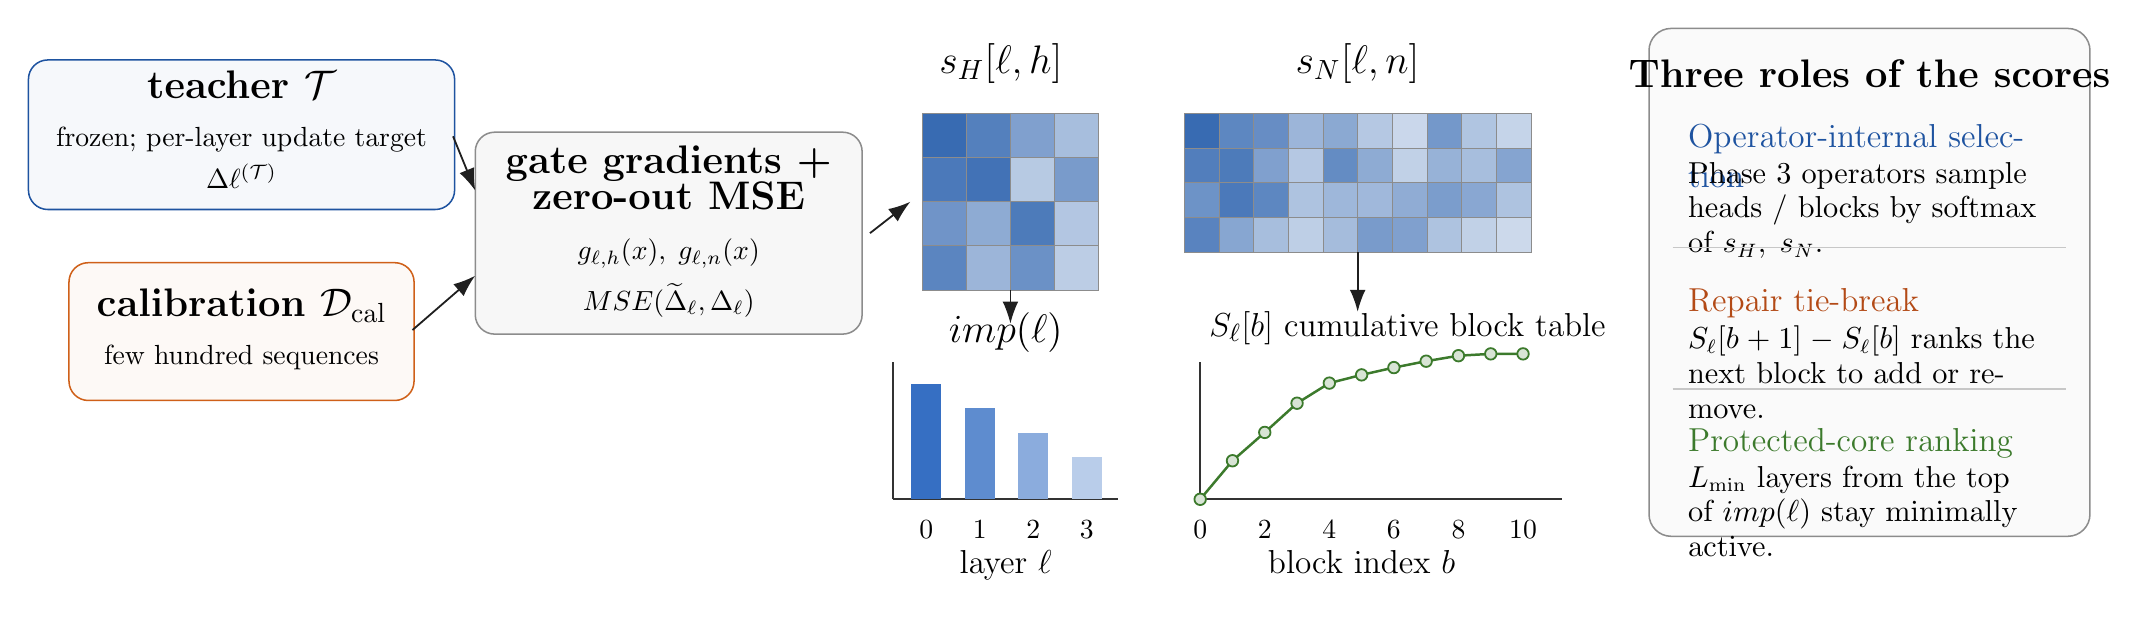
\begin{tikzpicture}[
  x=1cm,y=1cm,
  >=Latex,
  every node/.style={outer sep=0pt},
  arr/.style={-{Latex[length=2.8mm,width=2.0mm]}, line width=0.65pt, draw=black!88},
  axis/.style={line width=0.65pt, draw=black!80},
  thinsep/.style={line width=0.45pt, draw=black!22},
  sourcebox/.style={
    rounded corners=7pt,
    minimum width=4.35cm,
    minimum height=1.75cm,
    inner sep=4pt,
    align=center,
    font=\normalsize,
    line width=0.55pt
  },
  gatebox/.style={
    rounded corners=7pt,
    draw=black!45,
    fill=black!3,
    minimum width=4.10cm,
    minimum height=2.45cm,
    inner sep=5pt,
    align=center,
    font=\normalsize,
    line width=0.55pt
  },
  roleline/.style={font=\fontsize{10.7}{12.6}\selectfont, align=left, text width=4.70cm, anchor=north west},
  roletitle/.style={font=\bfseries\fontsize{14}{16}\selectfont, align=center, anchor=north},
  rolesection/.style={font=\fontsize{12.4}{14.4}\selectfont, align=left, text width=4.75cm, anchor=north west}
]

% Palette.
\definecolor{boxblue}{RGB}{30,83,160}
\definecolor{boxorange}{RGB}{207,96,25}
\definecolor{deepblue}{RGB}{24,83,166}
\definecolor{softblue}{RGB}{218,233,253}
\definecolor{plotblue}{RGB}{37,99,190}
\definecolor{plotgreen}{RGB}{60,122,44}
\definecolor{plotorange}{RGB}{179,74,22}

% -----------------------------------------------------------------------------
% Source boxes.
% -----------------------------------------------------------------------------
\node[sourcebox, draw=boxblue, fill=boxblue!4] (teacher) at (2.175,5.35) {%
  \begin{tabular}{c}
    {\bfseries\Large teacher $\mathcal{T}$}\\[1.8mm]
    frozen; per-layer update target\\[1.0mm]
    $\Delta\ell^{(\mathcal{T})}$
  \end{tabular}%
};

\node[sourcebox, draw=boxorange, fill=boxorange!4] (calib) at (2.175,2.85) {%
  \begin{tabular}{c}
    {\bfseries\Large calibration $\mathcal{D}_{\mathrm{cal}}$}\\[1.9mm]
    few hundred sequences
  \end{tabular}%
};

% -----------------------------------------------------------------------------
% Scoring block.
% -----------------------------------------------------------------------------
\node[gatebox] (gate) at (7.60,4.10) {%
  \begin{tabular}{c}
    {\bfseries\Large gate gradients +}\\[-0.2mm]
    {\bfseries\Large zero-out MSE}\\[2.2mm]
    $g_{\ell,h}(x),\; g_{\ell,n}(x)$\\[1.7mm]
    $\operatorname{MSE}(\widetilde{\Delta}_{\ell},\Delta_{\ell})$
  \end{tabular}%
};

\draw[arr] ([xshift=-0.02cm,yshift=-0.02cm]teacher.east) -- ([yshift=0.54cm]gate.west);
\draw[arr] ([xshift=-0.02cm,yshift=0.02cm]calib.east)   -- ([yshift=-0.54cm]gate.west);

% -----------------------------------------------------------------------------
% Heatmaps.  The values below are color intensities in [0,100].
% Larger values are drawn as darker blue cells.  Cell corners were calculated as:
%   x = top-left-x + column * cell-size,
%   y = top-left-y - row    * cell-size.
% Explicit cells are used so the file is robust in every LaTeX installation.
% -----------------------------------------------------------------------------

\newcommand{\HeatCell}[4]{%
  \path[draw=black!45, line width=0.22pt, fill=deepblue!#4!white]
    (#1,#2) rectangle ++(#3,-#3);%
}

% s_H heatmap: 4 layers x 4 heads shown schematically.
\def\hX{10.82}
\def\hY{5.62}
\def\hC{0.56}
\HeatCell{10.82}{5.62}{0.56}{86}
\HeatCell{11.38}{5.62}{0.56}{74}
\HeatCell{11.94}{5.62}{0.56}{55}
\HeatCell{12.50}{5.62}{0.56}{38}
\HeatCell{10.82}{5.06}{0.56}{78}
\HeatCell{11.38}{5.06}{0.56}{82}
\HeatCell{11.94}{5.06}{0.56}{31}
\HeatCell{12.50}{5.06}{0.56}{58}
\HeatCell{10.82}{4.50}{0.56}{62}
\HeatCell{11.38}{4.50}{0.56}{49}
\HeatCell{11.94}{4.50}{0.56}{77}
\HeatCell{12.50}{4.50}{0.56}{33}
\HeatCell{10.82}{3.94}{0.56}{71}
\HeatCell{11.38}{3.94}{0.56}{43}
\HeatCell{11.94}{3.94}{0.56}{64}
\HeatCell{12.50}{3.94}{0.56}{29}

\node[font=\fontsize{13.8}{15}\selectfont, anchor=south] at ($(\hX+1.0,\hY+0.27)$) {$s_H[\ell,h]$};

% s_N heatmap: 4 layers x 10 neuron blocks shown schematically.
\def\nX{14.15}
\def\nY{5.62}
\def\nC{0.44}
\HeatCell{14.15}{5.62}{0.44}{86}
\HeatCell{14.59}{5.62}{0.44}{70}
\HeatCell{15.03}{5.62}{0.44}{66}
\HeatCell{15.47}{5.62}{0.44}{43}
\HeatCell{15.91}{5.62}{0.44}{50}
\HeatCell{16.35}{5.62}{0.44}{32}
\HeatCell{16.79}{5.62}{0.44}{23}
\HeatCell{17.23}{5.62}{0.44}{60}
\HeatCell{17.67}{5.62}{0.44}{34}
\HeatCell{18.11}{5.62}{0.44}{25}
\HeatCell{14.15}{5.18}{0.44}{75}
\HeatCell{14.59}{5.18}{0.44}{77}
\HeatCell{15.03}{5.18}{0.44}{55}
\HeatCell{15.47}{5.18}{0.44}{32}
\HeatCell{15.91}{5.18}{0.44}{67}
\HeatCell{16.35}{5.18}{0.44}{49}
\HeatCell{16.79}{5.18}{0.44}{27}
\HeatCell{17.23}{5.18}{0.44}{45}
\HeatCell{17.67}{5.18}{0.44}{38}
\HeatCell{18.11}{5.18}{0.44}{53}
\HeatCell{14.15}{4.74}{0.44}{63}
\HeatCell{14.59}{4.74}{0.44}{78}
\HeatCell{15.03}{4.74}{0.44}{70}
\HeatCell{15.47}{4.74}{0.44}{35}
\HeatCell{15.91}{4.74}{0.44}{42}
\HeatCell{16.35}{4.74}{0.44}{41}
\HeatCell{16.79}{4.74}{0.44}{48}
\HeatCell{17.23}{4.74}{0.44}{57}
\HeatCell{17.67}{4.74}{0.44}{51}
\HeatCell{18.11}{4.74}{0.44}{35}
\HeatCell{14.15}{4.30}{0.44}{72}
\HeatCell{14.59}{4.30}{0.44}{52}
\HeatCell{15.03}{4.30}{0.44}{38}
\HeatCell{15.47}{4.30}{0.44}{28}
\HeatCell{15.91}{4.30}{0.44}{39}
\HeatCell{16.35}{4.30}{0.44}{58}
\HeatCell{16.79}{4.30}{0.44}{55}
\HeatCell{17.23}{4.30}{0.44}{35}
\HeatCell{17.67}{4.30}{0.44}{27}
\HeatCell{18.11}{4.30}{0.44}{22}

\node[font=\fontsize{13.8}{15}\selectfont, anchor=south] at ($(\nX+2.20,\nY+0.27)$) {$s_N[\ell,n]$};

\draw[arr] ([xshift=0.10cm]gate.east) -- (\hX-0.15,\hY-1.12);

% Down arrows from score tables to their derived summaries.
\draw[arr] ($(\hX+1.12,\hY-2.24)$) -- ($(\hX+1.12,2.95)$);
\draw[arr] ($(\nX+2.20,\nY-1.76)$) -- ($(\nX+2.20,3.1)$);

% -----------------------------------------------------------------------------
% Layer importance bar chart.
% -----------------------------------------------------------------------------
\def\bX{10.45}
\def\bY{0.72}
\def\bW{2.85}
\def\bH{1.75}

\draw[axis] (\bX,\bY) -- ++(\bW,0);
\draw[axis] (\bX,\bY) -- ++(0,\bH);
\node[font=\fontsize{13.4}{9}\selectfont, anchor=south] at ($(\bX+1.43,\bY+\bH)$) {$imp(\ell)$};

% Bar geometry: center step 0.68 cm, width 0.38 cm.
\foreach \i/\height/\shade in {0/1.47/92,1/1.16/74,2/0.84/53,3/0.54/32}{%
  \pgfmathsetmacro{\barcx}{\bX + 0.42 + \i*0.68}%
  \path[fill=plotblue!\shade!white, draw=none]
    ($(\barcx-0.19,\bY)$) rectangle ++(0.38,\height);
  \node[font=\fontsize{10.4}{12}\selectfont, anchor=north] at (\barcx,\bY-0.15) {\i};
}
\node[font=\fontsize{11.5}{13}\selectfont, anchor=north] at ($(\bX+1.43,\bY-0.53)$) {layer $\ell$};

% -----------------------------------------------------------------------------
% Cumulative block table plot.
% -----------------------------------------------------------------------------
\def\cX{14.35}
\def\cY{0.72}
\def\cW{4.60}
\def\cH{1.75}
\def\dx{0.41}
\def\ys{1.16}

\draw[axis] (\cX,\cY) -- ++(\cW,0);
\draw[axis] (\cX,\cY) -- ++(0,\cH);
\node[
  font=\fontsize{12.5}{15}\selectfont,
  anchor=south west
] at ($(\cX,\cY+\cH+0.1)$) {$S_{\ell}[b]$ cumulative block table};

% Draw line by explicit cumulative values. Mapping: y = cY + 0.13 + ys * value.
\coordinate (p0)  at ($(\cX+0*\dx,\cY+0.0+0.00*\ys)$);
\coordinate (p1)  at ($(\cX+1*\dx,\cY+0.13+0.31*\ys)$);
\coordinate (p2)  at ($(\cX+2*\dx,\cY+0.13+0.62*\ys)$);
\coordinate (p3)  at ($(\cX+3*\dx,\cY+0.13+0.94*\ys)$);
\coordinate (p4)  at ($(\cX+4*\dx,\cY+0.13+1.16*\ys)$);
\coordinate (p5)  at ($(\cX+5*\dx,\cY+0.13+1.25*\ys)$);
\coordinate (p6)  at ($(\cX+6*\dx,\cY+0.13+1.33*\ys)$);
\coordinate (p7)  at ($(\cX+7*\dx,\cY+0.13+1.40*\ys)$);
\coordinate (p8)  at ($(\cX+8*\dx,\cY+0.13+1.46*\ys)$);
\coordinate (p9)  at ($(\cX+9*\dx,\cY+0.13+1.48*\ys)$);
\coordinate (p10) at ($(\cX+10*\dx,\cY+0.13+1.48*\ys)$);

\draw[plotgreen, line width=0.9pt]
  (p0)--(p1)--(p2)--(p3)--(p4)--(p5)--(p6)--(p7)--(p8)--(p9)--(p10);
\foreach \p in {p0,p1,p2,p3,p4,p5,p6,p7,p8,p9,p10}{%
  \filldraw[fill=plotgreen!20!white, draw=plotgreen, line width=0.65pt] (\p) circle[radius=0.073];
}

\foreach \tick in {0,2,4,6,8,10}{%
  \pgfmathsetmacro{\tx}{\cX+\tick*\dx}%
  \node[font=\fontsize{10.4}{12}\selectfont, anchor=north] at (\tx,\cY-0.15) {\tick};
}
\node[font=\fontsize{11.5}{13}\selectfont, anchor=north] at ($(\cX+2.05,\cY-0.53)$) {block index $b$};

% -----------------------------------------------------------------------------
% Right explanation panel.
% -----------------------------------------------------------------------------
\def\rX{20.05}
\def\rY{0.25}
\def\rW{5.60}
\def\rH{6.45}
\path[draw=black!45, fill=black!2, line width=0.55pt, rounded corners=8pt]
  (\rX,\rY) rectangle ++(\rW,\rH);

\node[roletitle] at ($(\rX+0.5*\rW,\rY+\rH-0.28)$) {Three roles of the scores};

\node[rolesection, text=boxblue] at ($(\rX+0.38,\rY+\rH-1.10)$) {Operator-internal selection};
\node[roleline] at ($(\rX+0.38,\rY+\rH-1.58)$) {Phase 3 operators sample heads / blocks by softmax of $s_H,\;s_N$.};

\draw[thinsep] ($(\rX+0.30,\rY+\rH-2.78)$) -- ($(\rX+\rW-0.30,\rY+\rH-2.78)$);

\node[rolesection, text=plotorange] at ($(\rX+0.38,\rY+\rH-3.18)$) {Repair tie-break};
\node[roleline] at ($(\rX+0.38,\rY+\rH-3.66)$) {$S_{\ell}[b+1]-S_{\ell}[b]$ ranks the next block to add or remove.};

\draw[thinsep] ($(\rX+0.30,\rY+\rH-4.58)$) -- ($(\rX+\rW-0.30,\rY+\rH-4.58)$);

\node[rolesection, text=plotgreen] at ($(\rX+0.38,\rY+\rH-4.96)$) {Protected-core ranking};
\node[roleline] at ($(\rX+0.38,\rY+\rH-5.44)$) {$L_{\min}$ layers from the top of $imp(\ell)$ stay minimally active.};

\end{tikzpicture}
\end{document}
